% Author: Alejandro Santomé Valverde

\chapter{System-Level Applications and Network Architectures}\label{chap:apps} % (fold)

\section{Introduction: From the Chip to the Optical Network}\label{sec:ch5_intro}

Transitioning from the kilo-scale programmable photonic integrated circuit detailed in Chapter 4, 
the focus now shifts toward its functional application within modern optical communications. While 
the full-scale smart transceiver undergoes the final stages of heterogeneous packaging, validating 
its foundational optical concepts and exploring its topological impact on network architectures 
remain critical imperatives. Consequently, this chapter bridges the gap between hardware design and 
system-level implementation, projecting the capabilities of programmable photonics from fundamental 
component emulation up to massive core-network switching nodes.

Section \ref{sec:pol_diversity} establishes the experimental baseline by presenting the empirical 
characterization of the core polarization diversity subsystem. Utilizing a dedicated test structure 
that perfectly mirrors the functional path of the main transceiver—comprising edge couplers, 
polarization splitter and rotators, and a central programmable unit cell—this section validates the 
hardware's dynamic response. Through the application of variable optical delays, the experimental 
assessment demonstrates the subsystem's impact on standard, high-speed data traffic, explicitly 
evaluating Local Area Network Wavelength Division Multiplexing (LWDM)\cite{ieee_lwdm}, Coarse 
Wavelength Division Multiplexing (CWDM)\cite{itut_g694_2}, and Datacenter Reach 4-lane (DR4) 
\cite{ieee_dr4} communication standards.

Projecting these validated building blocks into complex network topologies, Section 
\ref{sec:switching_nodes} investigates the strategic role of the smart transceiver within 
next-generation optical switching nodes. Leveraging architectural frameworks derived from European 
collaborative projects, this theoretical analysis evaluates the insertion of the kilo-scale photonic 
mesh into both \textit{Route-and-Select} and \textit{Broadcast-and-Select} configurations, 
demonstrating its potential to revolutionize dynamic capacity allocation and spectral management.

Finally, Section \ref{sec:multicast} broadens the scope to massive Optical Circuit Switches (OCS) 
to address the ultimate challenge of spatial scalability and point-to-multipoint signal distribution.
Building upon the spatial routing principles established by the hexagonal meshes in the previous 
chapter, a highly scalable $32 \times 32$ OCS operating in the O-band is evaluated. This study 
specifically explores high-efficiency multicasting capabilities, discussing the current physical 
limitations and the necessary architectural improvements to approach a fully non-blocking 
$1 \times 32$ optical distribution.

\section{Experimental Emulation of the Polarization Diversity Core}\label{sec:pol_diversity}

To empirically evaluate the impact of differential group delay within the polarization diversity 
scheme, a dedicated test structure was designed and fabricated. As depicted in Figure 
\ref{fig:ch5-pol_div_test_str}, the layout comprises four parallel variants of the core 
polarization subsystem. Each variant consists of an input Edge Coupler, a Polarization 
Splitter-Rotator, a central Programmable Unit Cell coupled with a Phase Shifter , a Polarization 
Rotator-Combiner (PRC), and an output EC. The fundamental difference among the four structures 
lies in the engineered on-chip delay lines introduced immediately after the PSR. Specifically, the 
path length differences ($\Delta L$) between the upper and lower arms are set to 0 µm, 700 µm, 
3500 µm, and 7000 µm. These physical length variations introduce approximate temporal delays of 
0 ps, 10 ps, 50 ps, and 100 ps, respectively, providing a systematic framework to assess 
delay-induced signal degradation.

\begin{figure}[htbp]
    \centering
    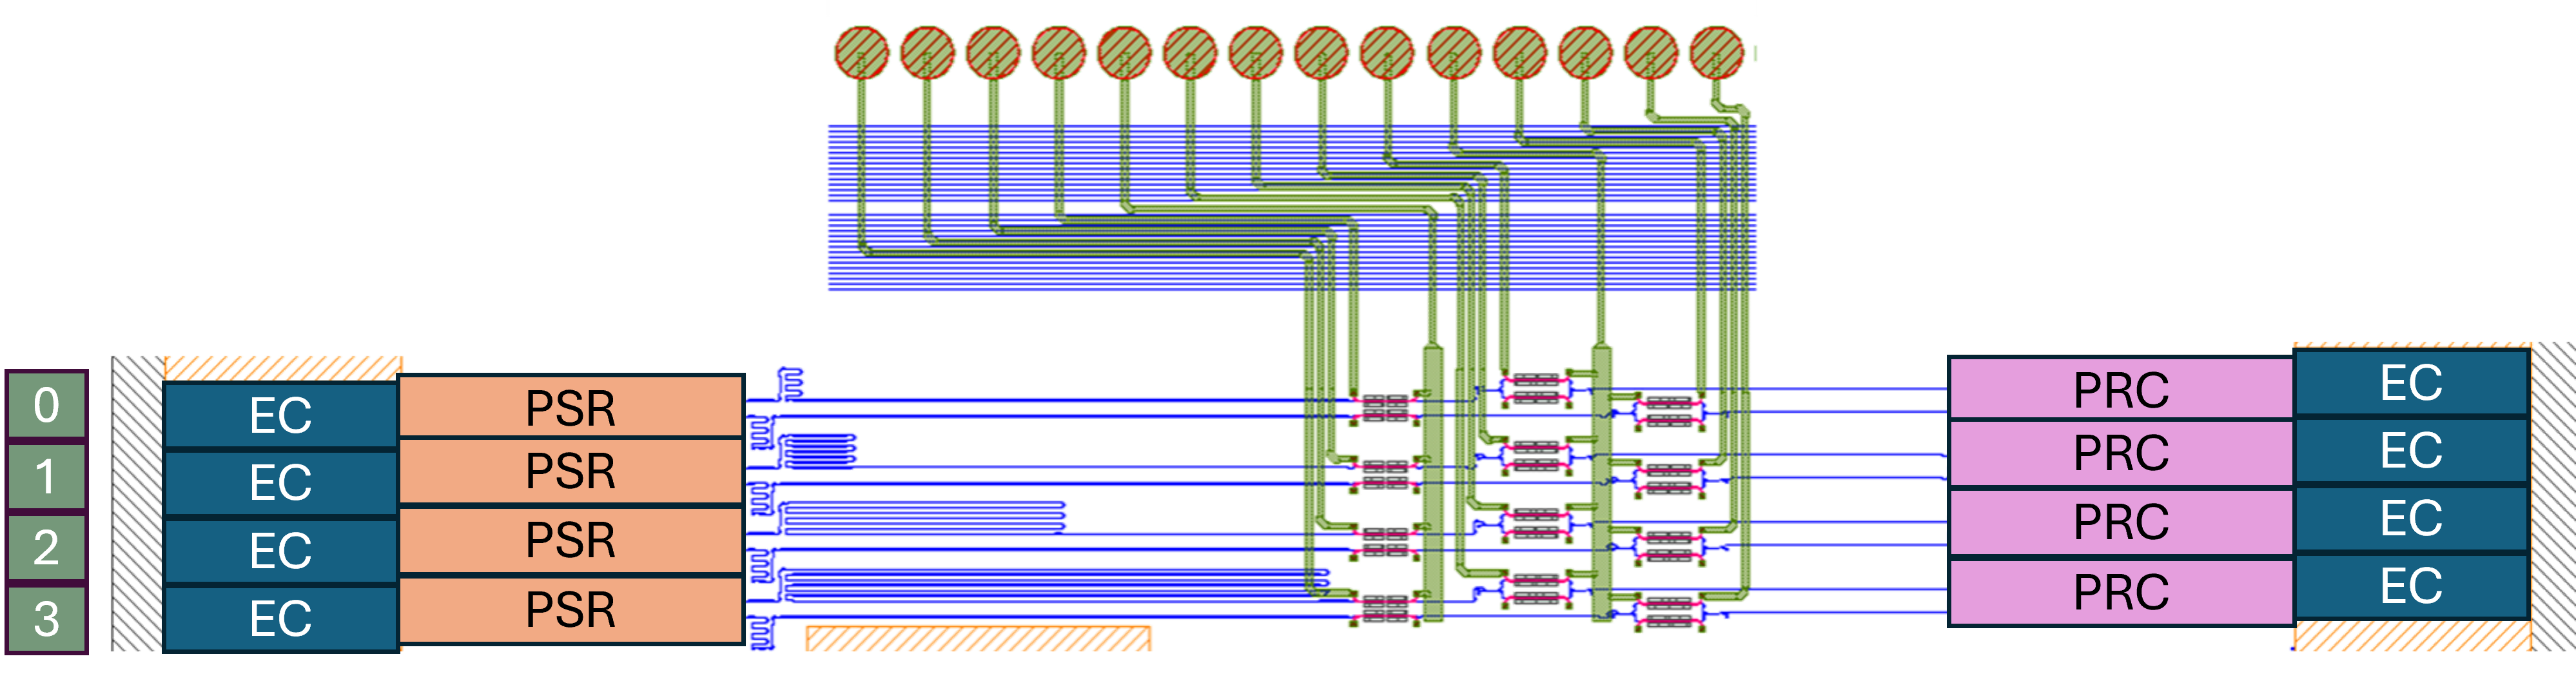
\includegraphics[width=\textwidth]{figures/ch5-pol_div_test_str.png} 
    \caption{Layout of the polarization diversity test structures. The diagram highlights four 
    parallel evaluation paths (0 to 3), each featuring an input EC, a PSR, variable on-chip delay 
    lines, a central PUC/PS stage, a PRC, and an output EC.}
    \label{fig:ch5-pol_div_test_str}
\end{figure}


The experimental testbed was designed to emulate realistic, high-capacity network environments. 
Data generation was driven by a Bit Error Rate Tester (BERT) equipped with commercial 400GE 
transceiver modules. To cover a comprehensive range of standard data streams, the evaluation 
utilized co-polarized 400GE-LWDM, both co-polarized and non-co-polarized 400GE-CWDM, and DR4 
transmitters. To rigorously test the hardware's polarization handling capabilities, a polarization 
controller was inserted at the output of the transmitter. Prior to coupling the signal into the 
photonic integrated circuit, a polarimeter was employed to verify and calibrate the input State of 
Polarization (SOP). This precise pre-calibration enabled systematic measurements under three 
distinct injection scenarios: 100\% TE, 100\% TM, and a perfectly balanced 50-50\% TE-TM mixed 
state.

Physical light coupling was achieved using cleaved optical fibers aligned to the on-chip edge 
couplers. The alignment process was optimized on an optical table equipped with piezo-controlled 
micro-positioners, utilizing an Optical Power Meter (OPM) to provide real-time feedback and 
maximize insertion efficiency. To guarantee stable operating conditions and avoid thermal drift 
during the measurements, a Thermo-Electric Cooler (TEC) was used to firmly fix the chip 
temperature at 45°C. Finally, the active components of the test structure—namely the PUC and the 
phase shifters—were electrically driven via a multi-contact probe. Two independent current sources 
were employed to feed the upper and lower arms individually, ensuring highly precise and decoupled 
tuning of the subsystem.

To compensate for the inherent insertion losses of the test structure and the fiber-to-chip 
coupling interfaces, a Semiconductor Optical Amplifier (SOA) was placed at the output of the PIC. 
This stage boosts the optical signal to an optimal power level before it is fed back into the BERT 
receiver for error analysis. A comprehensive view of the experimental testbed is presented in 
Figure \ref{fig:ch5-pol_div_setup}, where a photograph of the laboratory environment is overlaid 
with the logical block diagram of the interconnected instruments.

\begin{figure}[htbp]
    \centering
    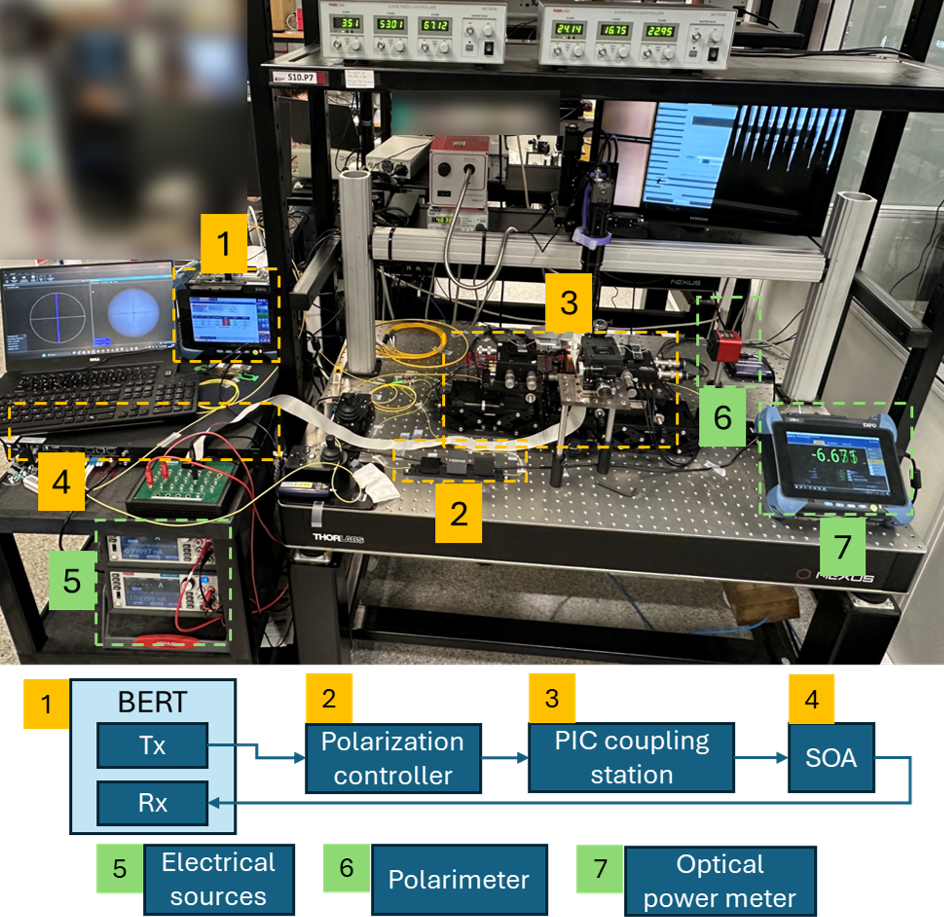
\includegraphics[width=\textwidth]{figures/ch5-pol_div_setup.png} 
    \caption{Experimental setup for the characterization of the polarization diversity subsystem. 
    Yellow boxes: key components in the signal path. Green boxes: standalone supporting modules.}
    \label{fig:ch5-pol_div_setup}
\end{figure}

\FloatBarrier

The rigorous pre-calibration of the input State of Polarization, performed prior to each 
measurement campaign, is visually confirmed in Figure \ref{fig:ch5-SOP}. Using the feedback from 
the polarimeter, the polarization controller was finely adjusted to generate the required test 
scenarios: purely TE modes ($0^\circ$ azimuth), purely TM modes ($90^\circ$ azimuth), and a 
perfectly balanced TE-TM mixed state ($45^\circ$ and $-45^\circ$ azimuth). As depicted, all 
calibrated states exhibit near-zero ellipticity, ensuring that the light launched into the edge 
couplers strictly adhered to the desired linear polarization conditions.

\begin{figure}[htbp]
    \centering
    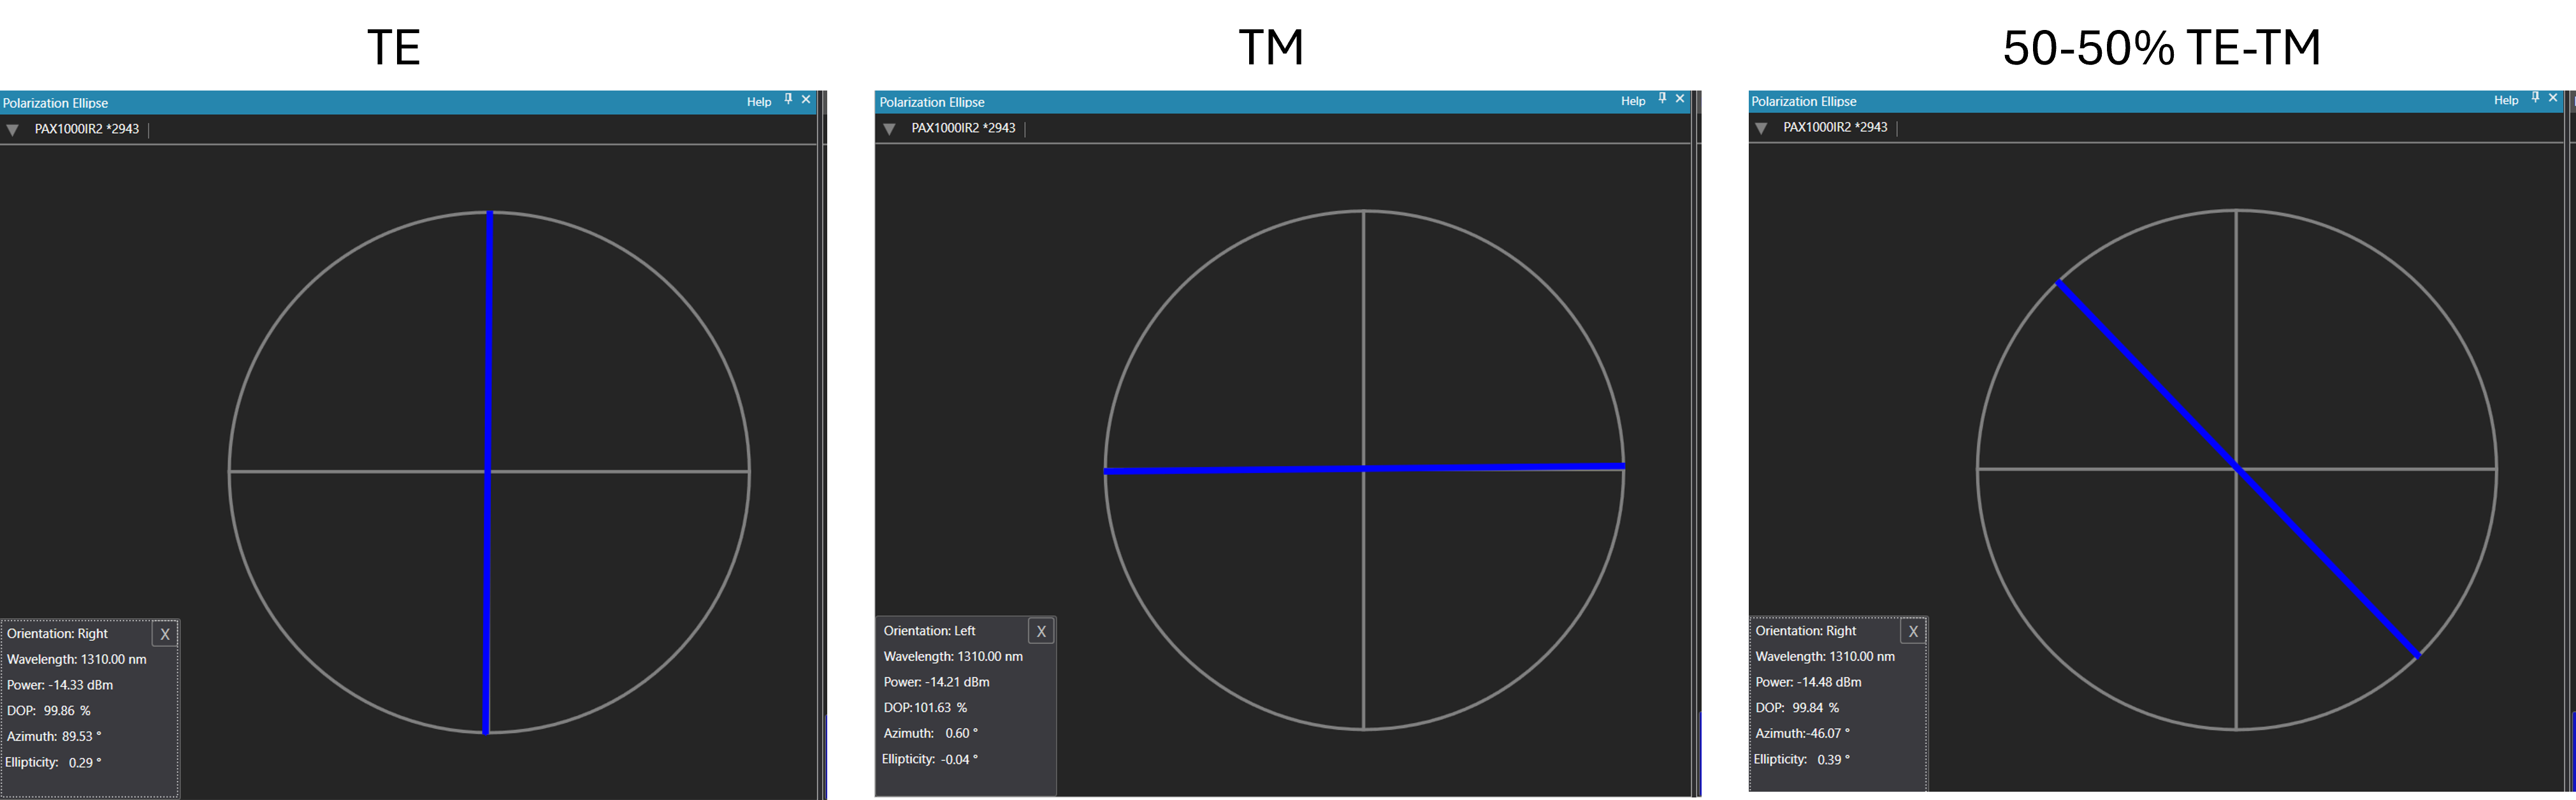
\includegraphics[width=\textwidth]{figures/ch5-SOP.png} 
    \caption{Measured polarization ellipses corresponding to the pre-calibrated input states: pure 
    TE ($0^\circ$ azimuth), pure TM ($90^\circ$ azimuth), and equally split TE-TM 
    ($\pm 45^\circ$ azimuth). All states successfully target $0^\circ$ ellipticity.}
    \label{fig:ch5-SOP}
\end{figure}


\subsection{Static Spectral Characterization}
\label{subsec:spectral_char}

Before assessing the dynamic performance with high-speed data streams, an initial static 
characterization was conducted to evaluate the continuous-wave (CW) optical response of the test 
structures. A tunable laser source was swept across the entire O-band, covering the wavelength 
range from 1260~nm to 1360~nm. This broad spectral sweep is essential to ensure that the baseline 
insertion losses and the wavelength-dependent behavior of the components (ECs, PSR, PUC, and PRC) 
are compatible with the wide grid of CWDM and the fine grid of LWDM standards.

The spectral responses were recorded for the four parallel structures, where $\Delta L = (0, 700, 
\allowbreak 3500, 7000)~\mu\mathrm{m}$ under the three pre-calibrated injection states. Firstly, 
each structure requires electrical tuning of the phase shifters to set the PUCs in their 
transmission maxima (specifically, for this test structure, the PUCs are configured in BAR state). 
The spectral results are compiled in Figure \ref{fig:ch5-pol_div_spectra}. For the purely 
co-polarized injection states, namely 100\% TE (a) and 100\% TM (b), the input light is 
predominantly routed through a single arm of the diversity circuit. Consequently, the transmission 
spectra primarily reflect the baseline insertion losses of the active optical path.
Conversely, the 50-50\% TE-TM mixed state (c) inherently excites both the upper and lower arms of 
the polarization subsystem simultaneously.  As expected, the optical power measured at the output
of each structure is very similar either using pure TE, pure TM or a 50-50 mixed state. This result
not only validates the structure but also reports low polarization-dependent loss (PDL). Note that
there is a noticeable ripple in all the traces independent of the SOP. This behavior is 
characteristic of a Fabry-Pérot cavity effect, caused by reflections at the chip facets when 
coupling cleaved fibers directly to the ECs. As the performance is predictable and stable for each 
wavelength, it does not imply any impairment in the transmission measurements discussed in the next 
section.

\begin{figure}[htpb]
    \centering
    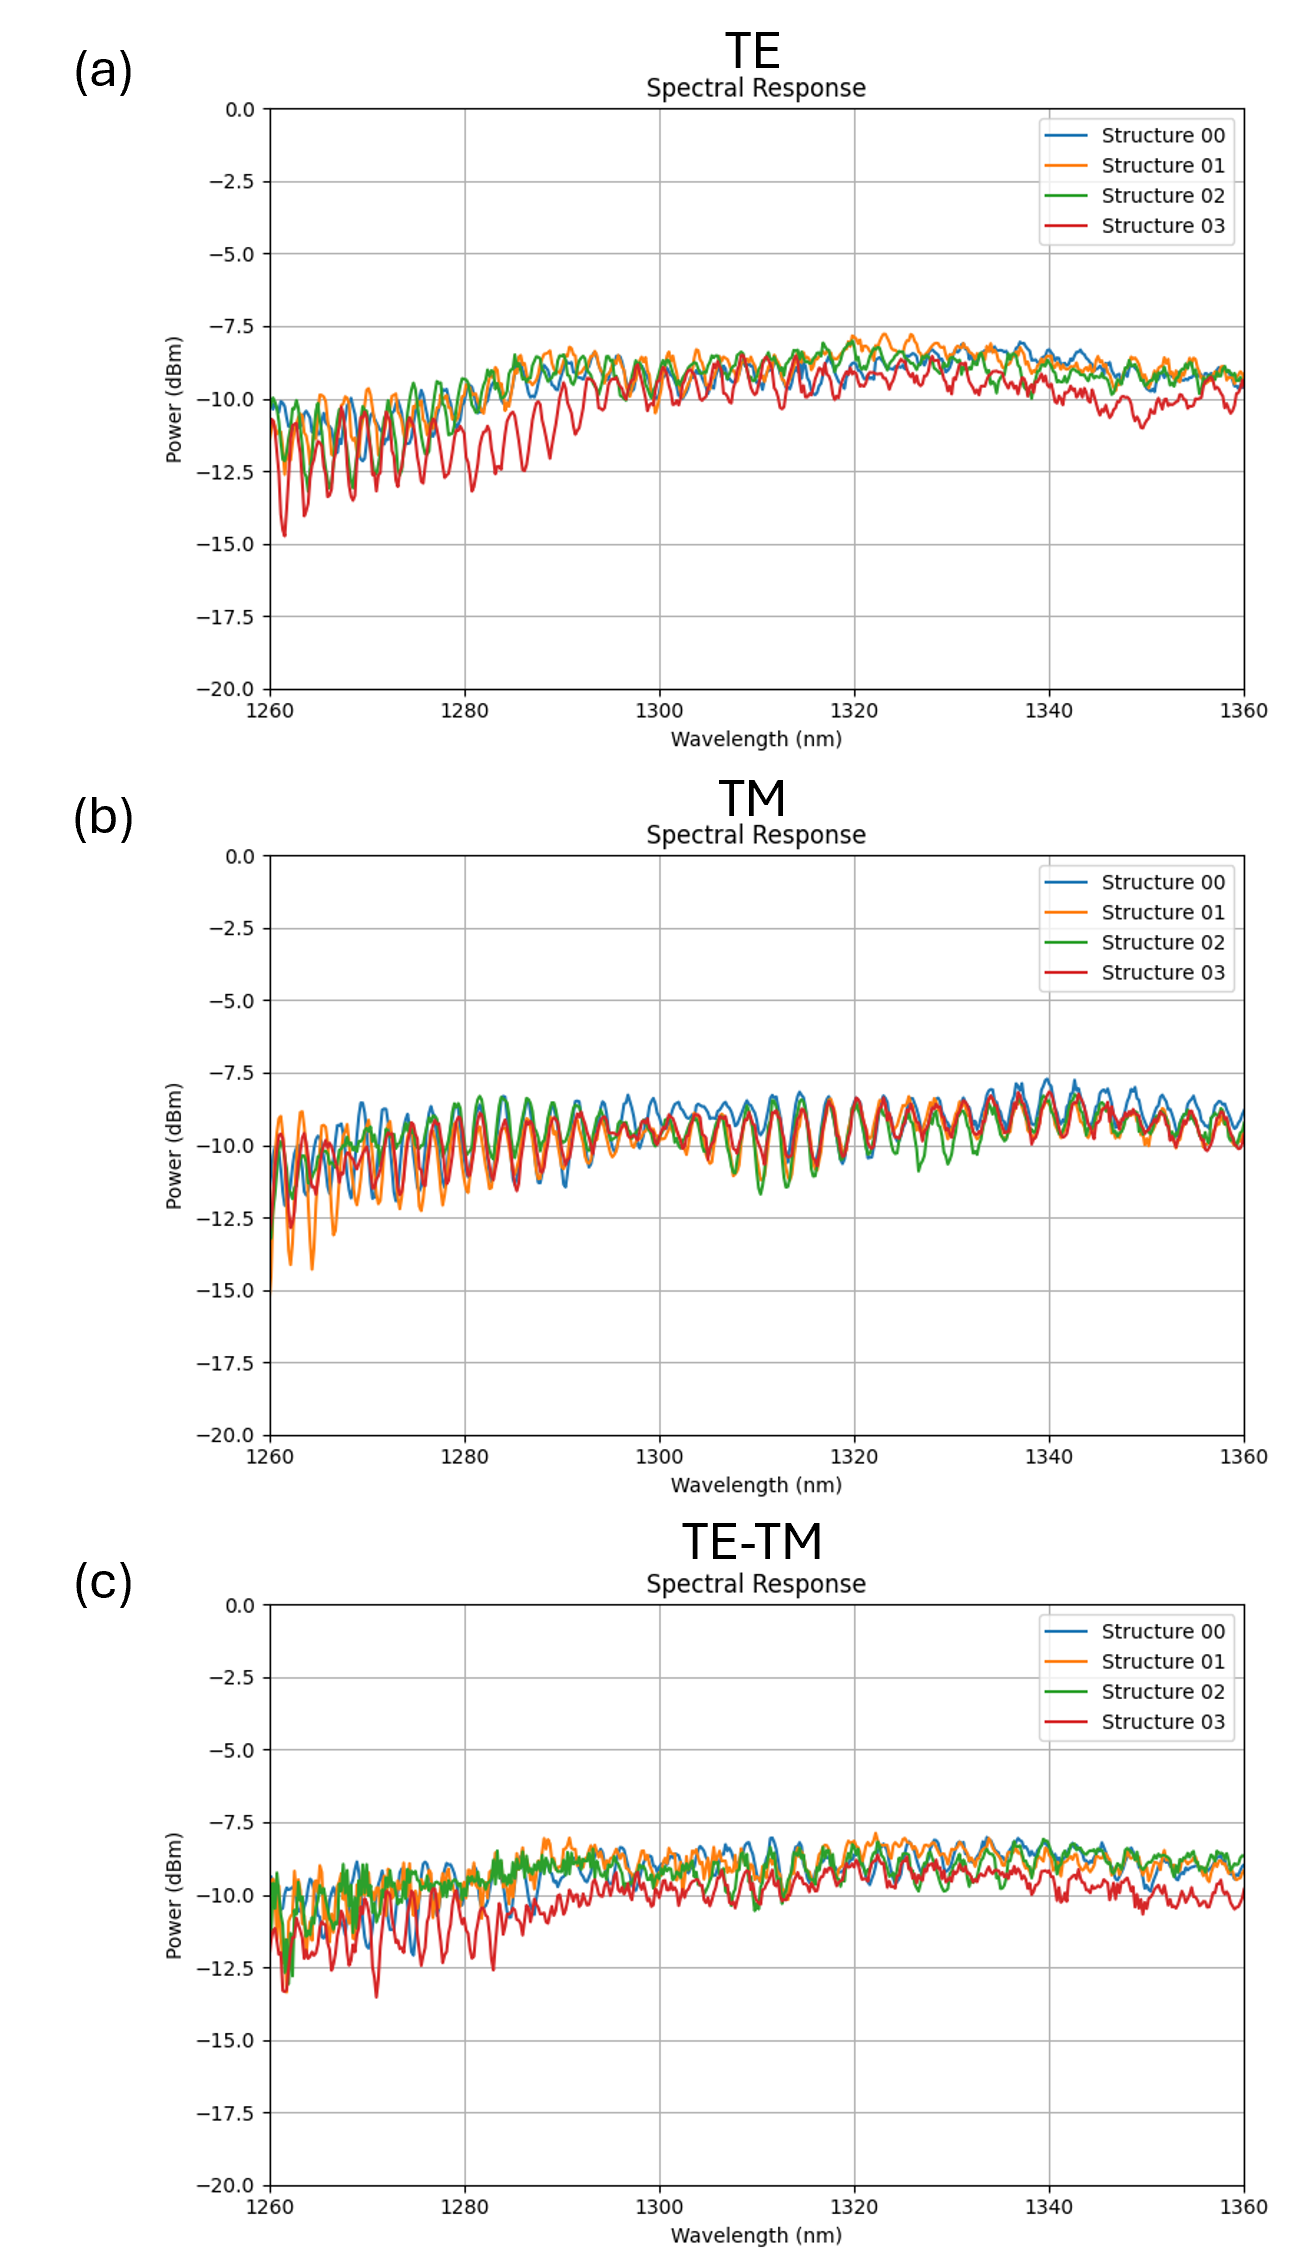
\includegraphics[width=0.74\textwidth]{figures/ch5-pol_div_spectra.png} 
    \caption{Static spectral characterization across the O-band (1260--1360~nm) of the four test 
    structures where $\Delta L = (0, 700, 3500, 7000)~\mu\mathrm{m}$. Transmission spectra are 
    shown for (a) pure TE injection, (b) pure TM injection, and (c) 50-50\% TE-TM mixed state.}
    \label{fig:ch5-pol_div_spectra}
\end{figure}

\FloatBarrier

\subsection{BER analysis}


\section{The Smart Transceiver in Next-Generation Switching Nodes}\label{sec:switching_nodes}

\section{Scaling up Routing Capabilities: Multicasting in O-Band OCS}\label{sec:multicast}

\section{Chapter Summary and Outlook}



% Si no me permiten usar Switching nodes
% 5.1 Introduction
% 5.2 Experimental Assessment of Polarization Diversity Dynamics
% 5.3 Advanced Spatial Routing: Multicasting Capabilities in Large-Scale Meshes

